\documentclass{article}

% If you're new to LaTeX, here's some short tutorials:
% https://www.overleaf.com/learn/latex/Learn_LaTeX_in_30_minutes
% https://en.wikibooks.org/wiki/LaTeX/Basics

% Formatting
\usepackage[utf8]{inputenc}
\usepackage[margin=1in]{geometry}
\usepackage[titletoc,title]{appendix}

% Math
% https://www.overleaf.com/learn/latex/Mathematical_expressions
% https://en.wikibooks.org/wiki/LaTeX/Mathematics
\usepackage{amsmath,amsfonts,amssymb,mathtools}

% Images
% https://www.overleaf.com/learn/latex/Inserting_Images
% https://en.wikibooks.org/wiki/LaTeX/Floats,_Figures_and_Captions
\usepackage{graphicx,float}

% Tables
% https://www.overleaf.com/learn/latex/Tables
% https://en.wikibooks.org/wiki/LaTeX/Tables

% Algorithms
% https://www.overleaf.com/learn/latex/algorithms
% https://en.wikibooks.org/wiki/LaTeX/Algorithms
\usepackage[ruled,vlined]{algorithm2e}
\usepackage{algorithmic}

% Code syntax highlighting
% https://www.overleaf.com/learn/latex/Code_Highlighting_with_minted
\usepackage{minted}
\usemintedstyle{borland}

% References
% https://www.overleaf.com/learn/latex/Bibliography_management_in_LaTeX
% https://en.wikibooks.org/wiki/LaTeX/Bibliography_Management
\usepackage{biblatex}
\addbibresource{references.bib}

% Title content
\title{CS6910 : Deep Learning (for Computer Vision)}
\author{\textbf{Irfaan Arif} \\ {\textbf{ME18B048}}}
\date{\textbf{Assignment 1}}

\begin{document}

\maketitle
\vspace{-2.6em}
\renewcommand{\abstractname}{\vspace{-\baselineskip}}
% Abstract
\begin{abstract}
    All experiments and results below are on the Dataset 5, mini-ImageNet with 33 classes 
\end{abstract}

% Introduction and Overview
\section{Part-A}
This part was to train a network for image classification on the given dataset and experiment with the following network parameters
\begin{enumerate}
    \item Number of Convolutional (conv) layers
    \item Number of fully connected (fc) layers
    \item The number of filters in different layers
    \item Maxpooling layers
    \item Training time (number of epochs)
    \item Stride in different layers
\end{enumerate}

\noindent
The models were trained on a AWS instance (g4dn.xlarge)  with \textbf{batch size 4} and for \textbf{100 epochs} with a learning rate\textbf{(lr) of 0.001} with SGD, and the remaining parameters same as the one in the boilerplate code. \\

\noindent
The model with the best validation accuracy among all the epochs was taken as the result for each experiment.

% Conv
\subsection{Number of Convolutional (conv) layers}
The boiler plate model was used as the baseline, and different models were trained by removing upto 2 conv layers or by adding upto 2 more conv layers. \\

\begin{figure}[H]
    \centering
    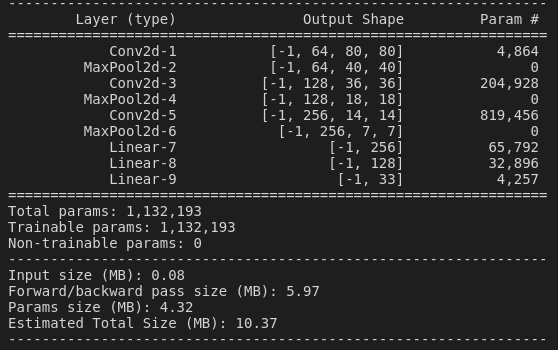
\includegraphics[width=0.60\linewidth]{conv/baseline_model.png}
    \caption{The baseline model with 3 convolutional layers}
    \label{fig:conv_base}
\end{figure}

\noindent
The baseline model as seen in Figure \ref{fig:conv_base} has 3 conv layers so we have a model with 1 conv layer at the lower end (Figure \ref{fig:conv_small}) and with 5 total conv layers at the other end (Figure \ref{fig:conv_big}). The numbers of output filters of some models were also adjusted to fit in with the fc layers. Also after every convolution layer, we are also doing maxpooling with a (2X2) kernel and stride 2.

\begin{figure}
\centering
\begin{minipage}{.5\linewidth}
  \centering
  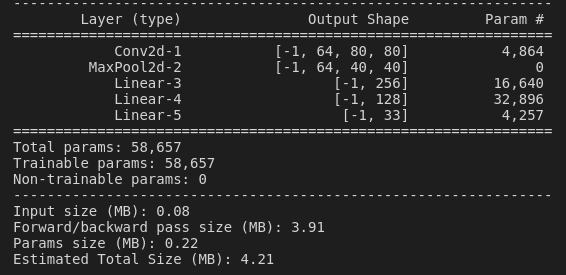
\includegraphics[width=.9\linewidth]{conv/conv_small.png}
  \caption{Model with 1 conv layer}
  \label{fig:conv_small}
\end{minipage}%
\begin{minipage}{.5\textwidth}
  \centering
  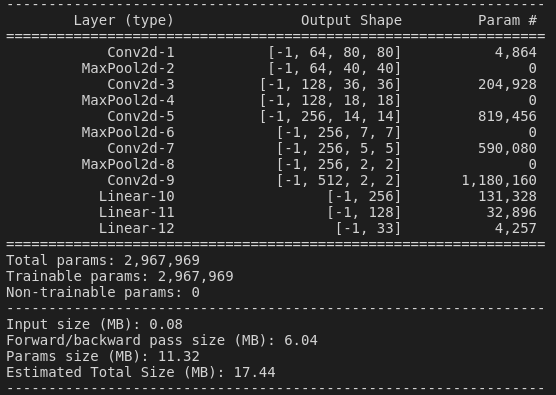
\includegraphics[width=.9\linewidth]{conv/conv_big.png}
  \caption{Model with 5 conv layers}
  \label{fig:conv_big}
\end{minipage}
\end{figure}


\begin{table}[h!]

\begin{center}
 \begin{tabular}{||c | c c c| c||} 
 
 \hline
\% Accuracy  &  Train &  Val & Test & No: of parameters\\ [0.5ex] 
 \hline\hline
 1 conv & 45.2 & 39.6 & 37.8 & 58657\\ 
 \hline
 2 conv & 74.6 & 52.3 & 50.7 & 279969\\
 \hline
 3 conv(baseline) & 94.1 & 59.6 & 58.5 & 1132193\\
 \hline
 4 conv & 92.0 & 56.7 & 56.4 & 1722273\\
 \hline
 5 conv & 93.2 & 56.7 & 57.1 & 2967969\\
 \hline

\end{tabular}
\end{center}
\vspace{-1.0em}
\caption{Accuracy of models with different number of conv layers} 
\end{table}

\noindent
As can be seen from Table 1, in general as you increase the number of convolutional layers, we get better perfomance in train, val and test. However after a while you reach a point of diminishing returns wherein adding more conv layers may even slightly hurt the performance and result in very long training times as the number of parameters also increases.
\\

\noindent
Especially for the model with only 1 conv layer, we can understand that the model is under-fitting, and our model is not large enough to learn a good representation (refer Figure \ref{fig:conv_small_acc}).
\\

\noindent
However for the models with 4 and 5 conv layers, we can see that these models quickly overfit and get high training accuracy and low validation accuracy, this is because there are a large number of parameters and we only have a limited dataset to work with. Transfer learning or forms of regularization like dropout could help alleviate this problem as well as also getting more training data (refer Figure \ref{fig:conv_big_acc}).

\begin{figure}[H]
\centering
\begin{minipage}{.5\linewidth}
  \centering
  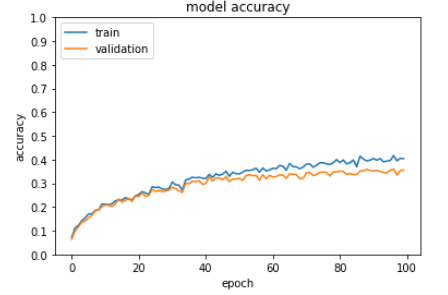
\includegraphics[width=.75\linewidth]{conv/conv_small_acc.png}
  \vspace{-1.0em}
  \caption{Model with 1 conv layer}
  \label{fig:conv_small_acc}
\end{minipage}%
\begin{minipage}{.5\textwidth}
  \centering
  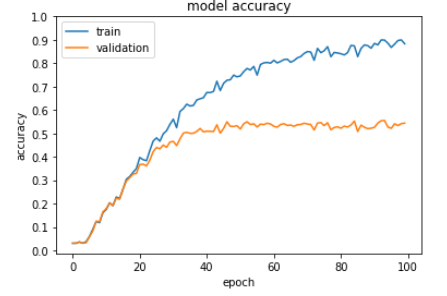
\includegraphics[width=.75\linewidth]{conv/conv_big_acc.png}
  \vspace{-1.0em}
  \caption{Model with 5 conv layers}
  \label{fig:conv_big_acc}
\end{minipage}
\end{figure}


% FC
\subsection{Number of fully connected (fc) layers}
Once again the boiler plate model was used as the baseline, and different models were trained by removing upto 1 fully connected layer or by adding upto 2 extra fully connected layers. \\

\noindent
Since the baseline model had 3 fc layers (including the final classification layer) we have models with 2 fc layers to ones with 5 fc layers in total.
As the number of fully connected layers are increased, the number of features in the linear layers were also appropriately increased. 

\begin{table}[h!]
\begin{center}
 \begin{tabular}{||c | c c c| c||} 
 
 \hline
\% Accuracy  &  Train &  Val & Test & No: of parameters\\ [0.5ex] 
 \hline\hline
 2 fc & 93.1 & 59.2 & 57.4 & 1066401\\
 \hline
 3 fc(baseline) & 91.5 & 59.6 & 57.9 & 1132193\\
 \hline
 4 fc & 93.4 & 59.4 & 59.5 & 1197985\\
 \hline
 5 fc & 89.8 & 58.5 & 57.8 & 1395105\\
 \hline
 
\end{tabular}
\end{center}
\label{table:fc_table}
\vspace{-1.0em}
\caption{Accuracy of models with different number of fully connected layers} 
\end{table}

\noindent
As can be seen from Table 2, there is not much variation when we change the number of fully connected layers. This could be due to the universal approximation theorem, in which the function mapping can be learned even if we only have 2 fc layers in feed forward style of sufficient width. 
\\

\begin{figure}[H]
    \centering
    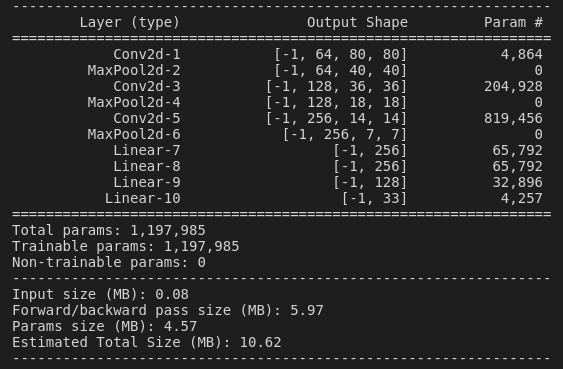
\includegraphics[width=0.60\linewidth]{fc/fc_best.png}
    \caption{The best model while changing FC layers}
    \label{fig:fc_best}
\end{figure}

\noindent
But more the width and number, a better approximation we can usually achieve, however since we have a limited dataset for this problem it is usually better to pick a medium sized network to minimize over-fitting.
Experimentally 4 fc layers (refer \ref{fig:fc_best} for the network) seems to work best for this particular problem, however the differences seem to be within the margin for error due to random weight initialization. 

% number of filters
\subsection{Number of filters in different layers}
For this part, 3 models were tested which had the general structure as the model in the boilerplate model. However the numbers of filters in both the convolutional and fully connected layers are vastly different in each model. \\

\begin{table}[h!]
\begin{center}
 \begin{tabular}{||c | c c c| c||} 
 
 \hline
\% Accuracy  &  Train &  Val & Test & No: of parameters\\ [0.5ex] 
 \hline\hline
 Net1 & 52.4 & 44.2 & 42.7 & 75347\\
 \hline
 Net2 & 81.3 & 53.2 & 51.6 & 682913\\
 \hline
 Net3 & 94.8 & 54.0 & 51.4 & 4967329\\
 \hline
 
\end{tabular}
\end{center}
\label{table:n_f_table}
\vspace{-1.0em}
\caption{Accuracy of models with different number of filters in layers} 
\end{table}

\noindent
Results obtained are shown in Table 3. We can also roughly call Net1 as a small model, Net2 as a medium sized model and Net3 as a large model.
\\

\noindent
As expected the small model seems to be under-fitting whereas the large model seems to definitely be over-fitting on the training dataset


\begin{figure}[H]
    \centering
    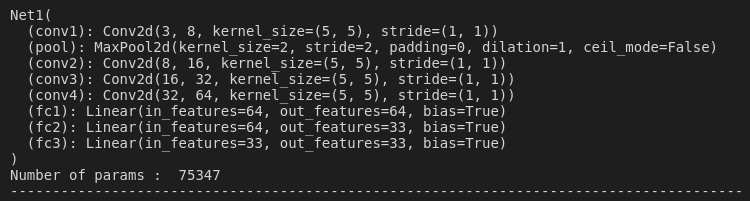
\includegraphics[width=0.80\linewidth]{n_f/n_f_1.png}
    \caption{Net1 - Small model}
    \label{fig:net1}
\end{figure}

\begin{figure} [H]
    \centering
    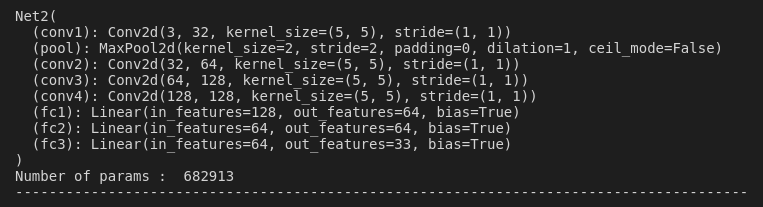
\includegraphics[width=0.80\linewidth]{n_f/n_f_2.png}
    \caption{Net2 - Medium sized model}
    \label{fig:net2}
\end{figure}

\begin{figure} [H]
    \centering
    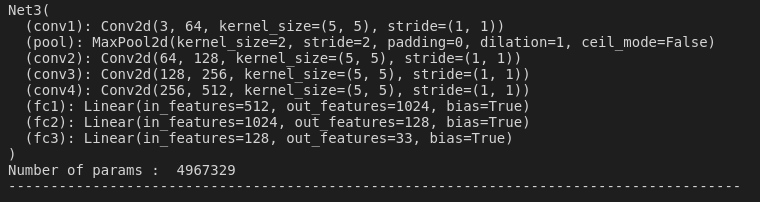
\includegraphics[width=0.80\linewidth]{n_f/n_f_3.png}
    \caption{Net3 - Large model}
    \label{fig:net3}
\end{figure}

\noindent
Another experiment that was run was to change the kernel size of the convolution layers, in general (3X3) and (5X5) gave almost same results for a majority of the different network architectures, while (7X7) and higher generally did worse. In general keeping the first convolutional layer kernel as larger seemed beneficial. 
\\
\\



% maxpooling
\subsection{Maxpooling layer}
For this part, 3 models were tested which various different structure/architecture for the model. The parameters and general structure of the model are derived from the basecase in the boilerplate code.

\noindent
Results obtained are shown in Table 4.

\begin{itemize}
    \item \textbf{Net1} : Without any maxpooling layer, instead using conv layers with a stride of 2 (ref Figure: \ref{fig:net1_max})
    \item \textbf{Net2} : Base case, maxpooling after every conv layer (ref Figure: \ref{fig:net2_max})
    \item \textbf{Net3} : Maxpooling after every 2 conv layers (ref Figure: \ref{fig:net3_max})
\end{itemize}

\begin{table}[h!]
\begin{center}
 \begin{tabular}{||c | c c c| c||} 
 
 \hline
\% Accuracy  &  Train &  Val & Test & No: of parameters\\ [0.5ex] 
 \hline\hline
 Net1 & 85.3 & 56.7 & 55.1 & 1132193\\
 \hline
 Net2 & 91.5 & 59.6 & 57.9 & 1132193 \\
 \hline
 Net3 & 90.2 & 63.1 & 62.4 & 4475041\\
 \hline
 
\end{tabular}
\end{center}
\label{table:maxpool_table}
\vspace{-1.0em}
\caption{Accuracy of the 3 different models} 
\end{table}

\begin{figure}[H]
    \centering
    \includegraphics[width=0.70\linewidth]{maxpool/maxpool_n1.png}
    \vspace{-1.0em}
    \caption{Net1 - No maxpool}
    \label{fig:net1_max}
\end{figure}

\begin{figure} [H]
    \centering
    \includegraphics[width=0.70\linewidth]{maxpool/maxpool_n2.png}
    \vspace{-1.0em}
    \caption{Net2 - Maxpool after every conv}
    \label{fig:net2_max}
\end{figure}

\begin{figure} [H]
    \centering
    \includegraphics[width=0.70\linewidth]{maxpool/maxpool_n3.png}
    \vspace{-1.0em}
    \caption{Net3 - Maxpool after every other conv}
    \label{fig:net3_max}
\end{figure}
\noindent
Net3 with maxpooling after every two convolutional layers is observed to be the clear winner here achieving a good test accuracy of 62\% although it a slightly large network.
\\

\noindent
Also changing the stride and kernel size of maxpooling layer produced inconsistent results, there was no general trend observed, it seemed to also depend on what the architecture was like and the parameters of the different layers. 

% Training time
\subsection{Training time (number of epochs)}
Note: The results for this section related to training time based on number of epochs was run on my local machine with a Nvidia Geforce 1060 GPU with an Intel i7-8750H CPU. Torch version was 1.6.0 with cuda 10.1, the process was profiled using the Nvidia Nsight Systems application.  
\\

\begin{figure}[H]
    \centering
    \includegraphics[width=0.90\linewidth]{gpu_utilization.png}
    \vspace{-1.0em}
    \caption{GPU utilization}
    \label{fig:gpu_util}
\end{figure}

\noindent
The GPU was being utilized almost throughout the time, peaking at 87\% utilization (Figure: \ref{fig:gpu_util}), GPU memory was not used much, therefore batch size could have been increased to get better training times.
\\

\begin{figure}[H]
    \centering
    \includegraphics[width=1.0\linewidth]{nsight_profiler.png}
    \vspace{-1.0em}
    \caption{Nsight profiling}
    \label{fig:nsight_profiling}
\end{figure}

\noindent 
There also does not seem to be any other major bottleneck in the system based on the profiling results (ref Figure: \ref{fig:nsight_profiling})
\\

\noindent
Training time is as such linear with the number of epochs, on average 1 epoch took 35.63 seconds with a standard deviation of 0.165 (ref Figure: \ref{fig:train_time})

\begin{figure}[H]
\centering
\begin{minipage}{.5\linewidth}
    \centering
    \includegraphics[width=0.9\linewidth]{train_times.png}
    \vspace{-1.0em}
    \caption{Training time}
    \label{fig:train_time}
\end{minipage}%
\begin{minipage}{.5\textwidth}
  \centering
  \includegraphics[width=.9\linewidth]{train_times_acc.png}
  \vspace{-1.0em}
  \caption{Accuracy's for 150 epochs}
  \label{fig:train_acc_comp}
\end{minipage}
\end{figure}

\noindent
However the validation loss plateaus at around around 100 epochs, and we can say to have completed training there, since going further would just mean overfitting on the train dataset (ref Figure: \ref{fig:train_acc_comp})

\begin{table}[h!]
\begin{center}
 \begin{tabular}{||c | c c ||} 
 
 \hline
\% Epoch number  &  Train &  Val\\ [0.5ex] 
 \hline\hline
 1 & 3 & 3\\
 \hline
 25 & 43.2 & 41.6\\
 \hline
 50 & 69.7 & 53.9\\
 \hline
 75 & 77.9 & 55.3\\
 \hline
 100 & 86.5 & 57.3\\
 \hline
 125 & 90.1 & 58.5\\
 \hline
 150 & 92.1 & 59.8\\
 \hline
 
\end{tabular}
\end{center}
\label{table:acc_train_times_tab}
\vspace{-1.0em}
\caption{Accuracy's(in \%) vs number of epochs}
\end{table}

% Strides
\subsection{Stride in different layers}
For stride in different layers, experiments were run mainly of changing the strides parameter in the convolutional layers, 3 cases were taken
\begin{itemize}
    \item \textbf{Net1} : Base case, as in the boilerplate code, with stride=1
    \item \textbf{Net2} : Setting stride=2, some maxpool layers were removed to accommodate this change
    \item \textbf{Net3} : Conv layers with stride=3, architecture was made different from the base case
\end{itemize}

\noindent
Results are shown in Table 6
\begin{table}[h!]
\begin{center}
 \begin{tabular}{||c | c c c||} 
 
 \hline
\% Accuracy  &  Train &  Val & Test\\ [0.5ex] 
 \hline\hline
  Net1 & 91.5 & 59.6 & 57.9\\
 \hline
 Net2 & 85.3 & 56.7 & 55.1\\
 \hline
 Net3 & 82.1 & 48.3 & 47.6\\
 \hline
 
\end{tabular}
\end{center}
\label{table:stride_table}
\vspace{-1.0em}
\caption{Accuracy of the 3 different models} 
\end{table}

\noindent
The results of variation of stride in the maxpooling layer has also been included in the Maxpooling layer subsection.


\subsection{Results}
After all the experiments and combining the best results of all the above, our final model achieved an accuracy of 63\% on the test dataset and its architecture is as shown in Figure \ref{fig:best_model}
\\

\noindent
One of the models in the maxpooling experiment (Net3, ref Fig: \ref{fig:net3_max}) has similar test accuracy, but it has around 4 times more parameters.
\\

\noindent
This model will be used in the next part of the assignment, the class-wise accuracy is also shown in Table 7.

\begin{figure}[H]
    \centering
    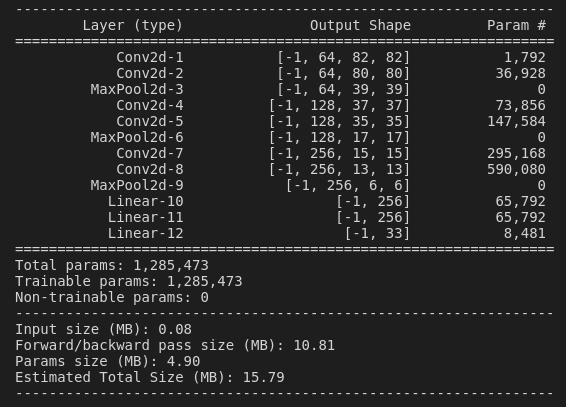
\includegraphics[width=0.60\linewidth]{best_model.png}
    \vspace{-1.0em}
    \caption{Best model (63\% test accuracy)}
    \label{fig:best_model}
\end{figure}

\begin{table} [H]
\begin{minipage}{0.5\textwidth}
\begin{tabular}{c|lc}
 & \textbf{Class name} & \textbf{\% Accuracy} \\
\hline
    0 & african hunting dog  &  77 \\
    1  &  ant  &  33 \\
    2  &  ashcan  &  31 \\
    3  &  black footed ferret  &  67 \\
    4  &  bookshop  &  37 \\
    5  &  carousel  &  49 \\
    6  &  catamaran  &  74 \\
    7  &  cocktail shaker  &  47 \\
    8  &  combination lock  &  38 \\
    9  &  consomme  &  78 \\
    10  &  coral reef  &  73 \\
    11  &  dalmatian  &  80 \\
    12  &  dishrag  &  66 \\
    13  &  fire screen  &  58 \\
    14  &  goose  &  58 \\
    15  &  green mamba  &  70 \\
    16  &  king crab  &  50 \\

% \vdots & \vdots & \vdots  \\ 
\end{tabular}

\end{minipage} \hfill
\begin{minipage}{0.5\textwidth}
\begin{tabular}{c|lc}
 & \textbf{Class name} & \textbf{\% Accuracy} \\
\hline
    17  &  ladybug  &  73 \\
    18  &  lion  &  82 \\
    19  &  lipstick  &  46 \\
    20  &  miniature poodle  &  59 \\
    21  &  orange  &  86 \\
    22  &  organ  &  70 \\
    23  &  parallel bars  &  37 \\
    24  &  photocopier  &  81 \\
    25  &  rhinoceros beetle  &  78 \\
    26  &  slot  &  81 \\
    27  &  snorkel  &  69 \\
    28  &  spider web  &  57 \\
    29  &  toucan  &  74 \\
    30  &  triceratops  &  56 \\
    31  &  unicycle  &  56 \\
    32  &  vase  &  31 \\
     &  &   \\
    
\end{tabular}
\end{minipage}
\caption{Class-wise accuracy}
\end{table}


%  Part B
\section{Part B}
We are going to be using the best model from Part A for all the remaining experiments (ref Fig \ref{fig:best_model})

\subsection{Occlusion sensitivity experiment}

For the occlusion sensitivity experiment, the results are based on using an (11X11) gray window being used to replace the content. The RGB value of the gray used to replace the content is taken as (211,211,211). 
\\

\noindent
If the class becomes different from the original prediction, then the confidence will be set as 0, no matter what the output of running the modified image through the model.
Also padding is not taken and at the edges a full (11X11) window will not be occluded/greyed out. The models outputs were softmaxed to get the probabilities.
\\

\noindent
The results obtained have been represented in the Figure \ref{fig:occ_sens}.

\noindent
Key takeaways based on the observations would be:
\begin{itemize}
    \item In general there are specific features that stand out and are learnt by the model such as an animals eyes, nose, beak,etc.
    \item For the classes that the model performed badly on, interesting it seems to be because the model is focusing/learning features of the background, hence hurting generalization.
    \item Edges of the class objects are a prominent feature and the confidence array seems to also be an outline of the object for most well performing classes.
    \item Classes with accuracy around or more than 80\% did not seem to be affected a lot by this experiment, as well as objets that cover a large part of the image, as expected from common intuition. As expected classes like the ladybug covering only small parts of the image, have sharp confidence decreases around the object position (ref Figure: \ref{fig:occ_sens_s1}).
\end{itemize}

\begin{figure}[H]
    \centering
    \includegraphics[width=1.0\linewidth]{occ_sens_final.png}
    \caption{Occlusion sensitivity experiment Results}
    \label{fig:occ_sens}
\end{figure}

\begin{figure}[H]
    \centering
    \includegraphics[width=0.4\linewidth]{occ_sens_bug1.jpg}
    \caption{Sharp confidence decreases on small sized class objects}
    \label{fig:occ_sens_s1}
\end{figure}

\subsection{Filter Analysis}

\subsubsection{Filter Identification}
2 filters each from the first 5 convolutional layers of our best model are taken for this part.
\\

\noindent
If we say that the N'th convolution layer in our model has n filters. We can choose any 2 random k'th filters in this conv layer for our filter analysis. This convolution layer has a receptive field depending on the number of preceding conv, max pool layers, and their kernel sizes.
\\

\noindent
For B test images of shape [B,3,H,W] (H=image height, W=image width), the response of the N'th conv layer is [B,n,h,w] (h=feature map height, w=feature map width). 
\\

\noindent
The response of k'th filter = output[:, k, :, :]. It has a size [B,h,w].
That is each image has a response of size [h,w] and each response at (i, j) for this array corresponds to a particular patch in the image (depending on the receptive field of the layer).
\\

\noindent
For for each image, we have hxw responses for each image. From this we now find the top-5 responses among responses from all the images. Here a response is defined as the value at (i,j) instead of something like taking norm of the entire activation. The receptive field and patch is calculated for each one of these top 5 and displayed.
\\

\noindent
Note : For all the figures below the above part shows the original image from which the image patch at the bottom is extracted from and the images are ordered from  left to right in decreasing order of responses.
\\

\begin{itemize}

\item \textbf{Conv layer 1} \\
\noindent
Conv layer 1 has 64 filters with a (3X3) kernel. The output after this layer is [64,82,82] and the receptive field is (3X3). The top 5 images corresponding to the maximum response are shown in Fig \ref{fig:l1_f1}, \ref{fig:l1_f2} and \ref{fig:l1_f3}. 
\begin{figure}[H]
    \centering
    \includegraphics[width=0.90\linewidth]{Filter_ident/L1/f1.png}
    \vspace{-1.0em}
    \caption{Layer1 - Filter 10}
    \label{fig:l1_f1}
\end{figure}
\begin{figure}[H]
    \centering
    \includegraphics[width=0.90\linewidth]{Filter_ident/L1/f2.png}
    \vspace{-1.0em}
    \caption{Layer1 - Filter 17}
    \label{fig:l1_f2}
\end{figure}
\begin{figure}[H]
    \centering
    \includegraphics[width=0.90\linewidth]{Filter_ident/L1/f3.png}
    \vspace{-1.0em}
    \caption{Layer1 - Filter 31}
    \label{fig:l1_f3}
\end{figure}

\item \textbf{Conv layer 2} \\
\noindent
Conv layer 2 also has 64 filters with a (3X3) kernel. The output after this layer is [64,80,80] and the receptive field for this layer is (5X5). The top 5 images corresponding to the maximum response are shown in Fig \ref{fig:l2_f1} and \ref{fig:l2_f2}. 
\begin{figure}[H]
    \centering
    \includegraphics[width=0.90\linewidth]{Filter_ident/L2/f1.png}
    \vspace{-1.0em}
    \caption{Layer2 - Filter 19}
    \label{fig:l2_f1}
\end{figure}
\begin{figure}[H]
    \centering
    \includegraphics[width=0.90\linewidth]{Filter_ident/L2/f2.png}
    \vspace{-1.0em}
    \caption{Layer2 - Filter 3}
    \label{fig:l2_f2}
\end{figure}

\item \textbf{Conv layer 3} \\
\noindent
The third convolutional layer has 128 filters with a (3X3) kernel once again. The output after this layer is [128,37,37] and the receptive field for this layer is (11X11). The top 5 images corresponding to the maximum response are shown in Fig \ref{fig:l3_f1} and \ref{fig:l1_f3}. 
\begin{figure}[H]
    \centering
    \includegraphics[width=0.90\linewidth]{Filter_ident/L3/f1.png}
    \vspace{-1.0em}
    \caption{Layer3 - Filter 7}
    \label{fig:l3_f1}
\end{figure}
\begin{figure}[H]
    \centering
    \includegraphics[width=0.90\linewidth]{Filter_ident/L3/f3.png}
    \vspace{-1.0em}
    \caption{Layer3 - Filter 36}
    \label{fig:l3_f3}
\end{figure}

\item \textbf{Conv layer 4} \\
\noindent
The fourth convolutional layer also has 128 filters with a (3X3) kernel once again. The output after this layer is [128,35,35] and the receptive field for this layer is (15X15). The top 5 images corresponding to the maximum response are shown in Fig \ref{fig:l4_f1} and \ref{fig:l4_f3}. 
\vspace{2.0em}
\begin{figure}[H]
    \centering
    \includegraphics[width=0.90\linewidth]{Filter_ident/L4/f1.png}
    \vspace{-1.0em}
    \caption{Layer4 - Filter 2}
    \label{fig:l4_f1}
\end{figure}
\vspace{2.0em}
\begin{figure}[H]
    \centering
    \includegraphics[width=0.90\linewidth]{Filter_ident/L4/f2.png}
    \vspace{-1.0em}
    \caption{Layer4 - Filter 4}
    \label{fig:l4_f3}
\end{figure}

There are quite some repeated imgs here but it because there are multiple lipsticks in the same image and the particular filter in Layer 5 which is filter 4 got activated at multiple (i,j) in the image.
\\

\newpage
\item \textbf{Conv layer 5} \\
\noindent
The fourth convolutional layer has 256 filters with a (3X3) kernel. The output after this layer is [256,15,15] and the receptive field for this layer is (25X25). The top 5 images corresponding to the maximum response are shown in Fig \ref{fig:l5_f1}, \ref{fig:l5_f2} and \ref{fig:l5_f3}. 
\begin{figure}[H]
    \centering
    \includegraphics[width=0.90\linewidth]{Filter_ident/L5/f1.png}
    \vspace{-1.0em}
    \caption{Layer5 - Filter 36}
    \label{fig:l5_f1}
\end{figure}
\begin{figure}[H]
    \centering
    \includegraphics[width=0.90\linewidth]{Filter_ident/L5/f2.png}
    \vspace{-1.0em}
    \caption{Layer5 - Filter 201}
    \label{fig:l5_f2}
\end{figure}
\begin{figure}[H]
    \centering
    \includegraphics[width=0.90\linewidth]{Filter_ident/L5/f3.png}
    \vspace{-1.0em}
    \caption{Layer5 - Filter 96}
    \label{fig:l5_f3}
\end{figure}

\end{itemize}

\subsubsection{Filter Modification}

For this part we will be individually turning off 10 filters from the above subsection (2 from each layer), i.e by making their weights zero. We are also only going to consider misses as those which were classified correctly before but start to mis-classify now.

\noindent
For each of the figures below, the top images are the mis-classifications int the first filter and the bottom images are the mis-classifications in the second filter.(random 10)

\begin{itemize}
    \item \textbf{Conv layer 1}
    
        Filter 10 and Filter 31
        \begin{figure}[H]
            \centering
            \includegraphics[width=1.0\linewidth]{Filter_off/layer1.png}
            \vspace{-2.0em}
            \caption{Mis-classifications in layer 1}
            \label{fig:l1_m1}
        \end{figure}

        \begin{table}[h!]
        \begin{center}
         \begin{tabular}{||c | c c c||}         
         \hline
        Filter tuned off & Initial accuracy  &  Number of misses &  New accuracy\\ [0.5ex] 
         \hline\hline
             Filter 10 & 64.0 & 50 & 62.5\\
             \hline
             Filter 31 & 64.0 & 12 & 63.7\\
         \hline
         \end{tabular}
        \end{center}
        \label{table:conv1_off}
        \vspace{-1.0em}
        \caption{Conv layer 1 filters turned off individually} 
        \end{table}


    \item \textbf{Conv layer 2}
    
        Filter 19 and Filter 3
        \begin{figure}[H]
            \centering
            \includegraphics[width=1.0\linewidth]{Filter_off/layer2.png}
            \vspace{-2.0em}
            \caption{Mis-classifications in layer 2}
            \label{fig:l2_m1}
        \end{figure}
        
        \begin{table}[h!]
        \begin{center}
         \begin{tabular}{||c | c c c||}         
         \hline
        Filter tuned off & Initial accuracy  &  Number of misses &  New accuracy\\ [0.5ex] 
         \hline\hline
             Filter 19 & 64.0 & 112 & 60.6\\
             \hline
             Filter 3 & 64.0 & 21 & 63.4\\
         \hline
         \end{tabular}
        \end{center}
        \label{table:conv2_off}
        \vspace{-1.0em}
        \caption{Conv layer 2 filters turned off individually} 
        \end{table}

\newpage       
    \item \textbf{Conv layer 3}
        
         Filter 7 and Filter 36
        
        \begin{figure}[H]
            \centering
            \includegraphics[width=1.0\linewidth]{Filter_off/layer3.png}
            \vspace{-2.0em}
            \caption{Mis-classifications in layer 3}
            \label{fig:l3_m1}
        \end{figure}
        
        \begin{table}[h!]
        \begin{center}
         \begin{tabular}{||c | c c c||}         
         \hline
        Filter tuned off & Initial accuracy  &  Number of misses &  New accuracy\\ [0.5ex] 
         \hline\hline
             Filter 7 & 64.0 & 27 & 63.2\\
             \hline
             Filter 36 & 64.0 & 30 & 63.1\\
         \hline
         \end{tabular}
        \end{center}
        \label{table:conv3_off}
        \vspace{-1.0em}
        \caption{Conv layer 3 filters turned off individually} 
        \end{table}
        
    \item \textbf{Conv layer 4}
    
        Filter 2 and Filter 4

        \begin{figure}[H]
            \centering
            \includegraphics[width=1.0\linewidth]{Filter_off/layer4.png}
            \vspace{-2.0em}
            \caption{Mis-classifications in layer 4}
            \label{fig:l4_m1}
        \end{figure}
        
        \begin{table}[h!]
        \begin{center}
         \begin{tabular}{||c | c c c||}         
         \hline
        Filter tuned off & Initial accuracy  &  Number of misses &  New accuracy\\ [0.5ex] 
         \hline\hline
             Filter 2 & 64.0 & 16 & 63.5\\
             \hline
             Filter 4 & 64.0 & 19 & 63.4\\
         \hline
         \end{tabular}
        \end{center}
        \label{table:conv4_off}
        \vspace{-1.0em}
        \caption{Conv layer 4 filters turned off individually} 
        \end{table}
\newpage       
        
    \item \textbf{Conv layer 5}
    
        Filter 201 and Filter 96
    
        \begin{figure}[H]
            \centering
            \includegraphics[width=1.0\linewidth]{Filter_off/layer5.png}
            \vspace{-2.0em}
            \caption{Mis-classifications in layer 5}
            \label{fig:l5_m1}
        \end{figure}
        
        \begin{table}[h!]
        \begin{center}
         \begin{tabular}{||c | c c c||}         
         \hline
        Filter tuned off & Initial accuracy  &  Number of misses &  New accuracy\\ [0.5ex] 
         \hline\hline
             Filter 201 & 64.0 & 16 & 63.5\\
             \hline
             Filter 96 & 64.0 & 8 & 63.8\\
         \hline
         \end{tabular}
        \end{center}
        \label{table:conv5_off}
        \vspace{-1.0em}
        \caption{Conv layer 5 filters turned off individually} 
        \end{table}


\end{itemize}
% \noindent


% Summary and Conclusions
\subsubsection{Summary and Conclusions}
From the filter identification experiment we can observe that the model at the earlier layers tends to focus on simple features like edges, corners , places where there are sharp gradient changes etc. However as you go into the deeper layer more information is being dimension-ally reduced down and represent in a lower form. The features here can be more general like eyes, body parts, shapes, etc. which are more complex and not easily representable. 
\\

\noindent
Switching off the filters also helps to further understand and infer what the model has really learnt and what features it is focussing on.

\end{document}
